\section{Main Results and Predictions}

Our theoretical model yields two central results with direct empirical implications for the persistence and variation of algorithmic bias. The analysis hinges on the firm's optimization problem, where we formally establish that the profit-maximizing value function, $V(b)$, is strictly concave (see Lemma 3 in the Appendix). This ensures a unique optimum for the level of bias, which we characterize below.

\begin{proposition}[Existence of Optimal Bias]
\label{prop:existence}
For any fairness-accuracy trade-off ($\kappa > 0$), a profit-maximizing firm's optimal choice of bias is strictly positive ($b^* > 0$).
\end{proposition}
\begin{proof}
See Appendix A.3. The proof shows that at zero bias, the marginal value of increasing bias is strictly positive ($dV/db|_{b=0} > 0$). Given the concavity of $V(b)$, the optimum must be greater than zero.
\end{proof}

This proposition provides our first key prediction: \textbf{Firms will rationally choose to employ biased algorithms even when groups have identical average productivity and debiasing is costless.} This outcome is not driven by animus or priors, but by the informational value gained from the precision-bias trade-off inherent in the technology.

\begin{proposition}[Comparative Static on the Trade-off]
\label{prop:comparative_static}
The optimal level of bias $b^*$ is increasing in the severity of the fairness-accuracy trade-off, $\kappa$.
\end{proposition}
\begin{proof}
See Appendix A.4. The proof uses the Implicit Function Theorem on the first-order condition to show that $\partial b^*/\partial\kappa > 0$.
\end{proof}

This result generates a set of powerful, testable predictions about where and why bias should vary. 
First, \textbf{firms or industries operating in environments with a steeper trade-off (a higher $\kappa$) will choose higher levels of bias, all else equal.} This might occur in contexts where prediction is inherently more complex or data is less balanced.
Second, and conversely, \textbf{technological improvements that flatten the fairness-accuracy trade-off (i.e., lower $\kappa$) should lead to measurable reductions in observed bias levels,} as the marginal benefit of retaining bias diminishes.

The model's mechanics and the intuition behind these results are summarized in Figure \ref{fig:main_results}, which is generated by the accompanying \texttt{results.py} script.

\begin{figure}[H]
    \centering
    % The path is relative from the main document's directory
    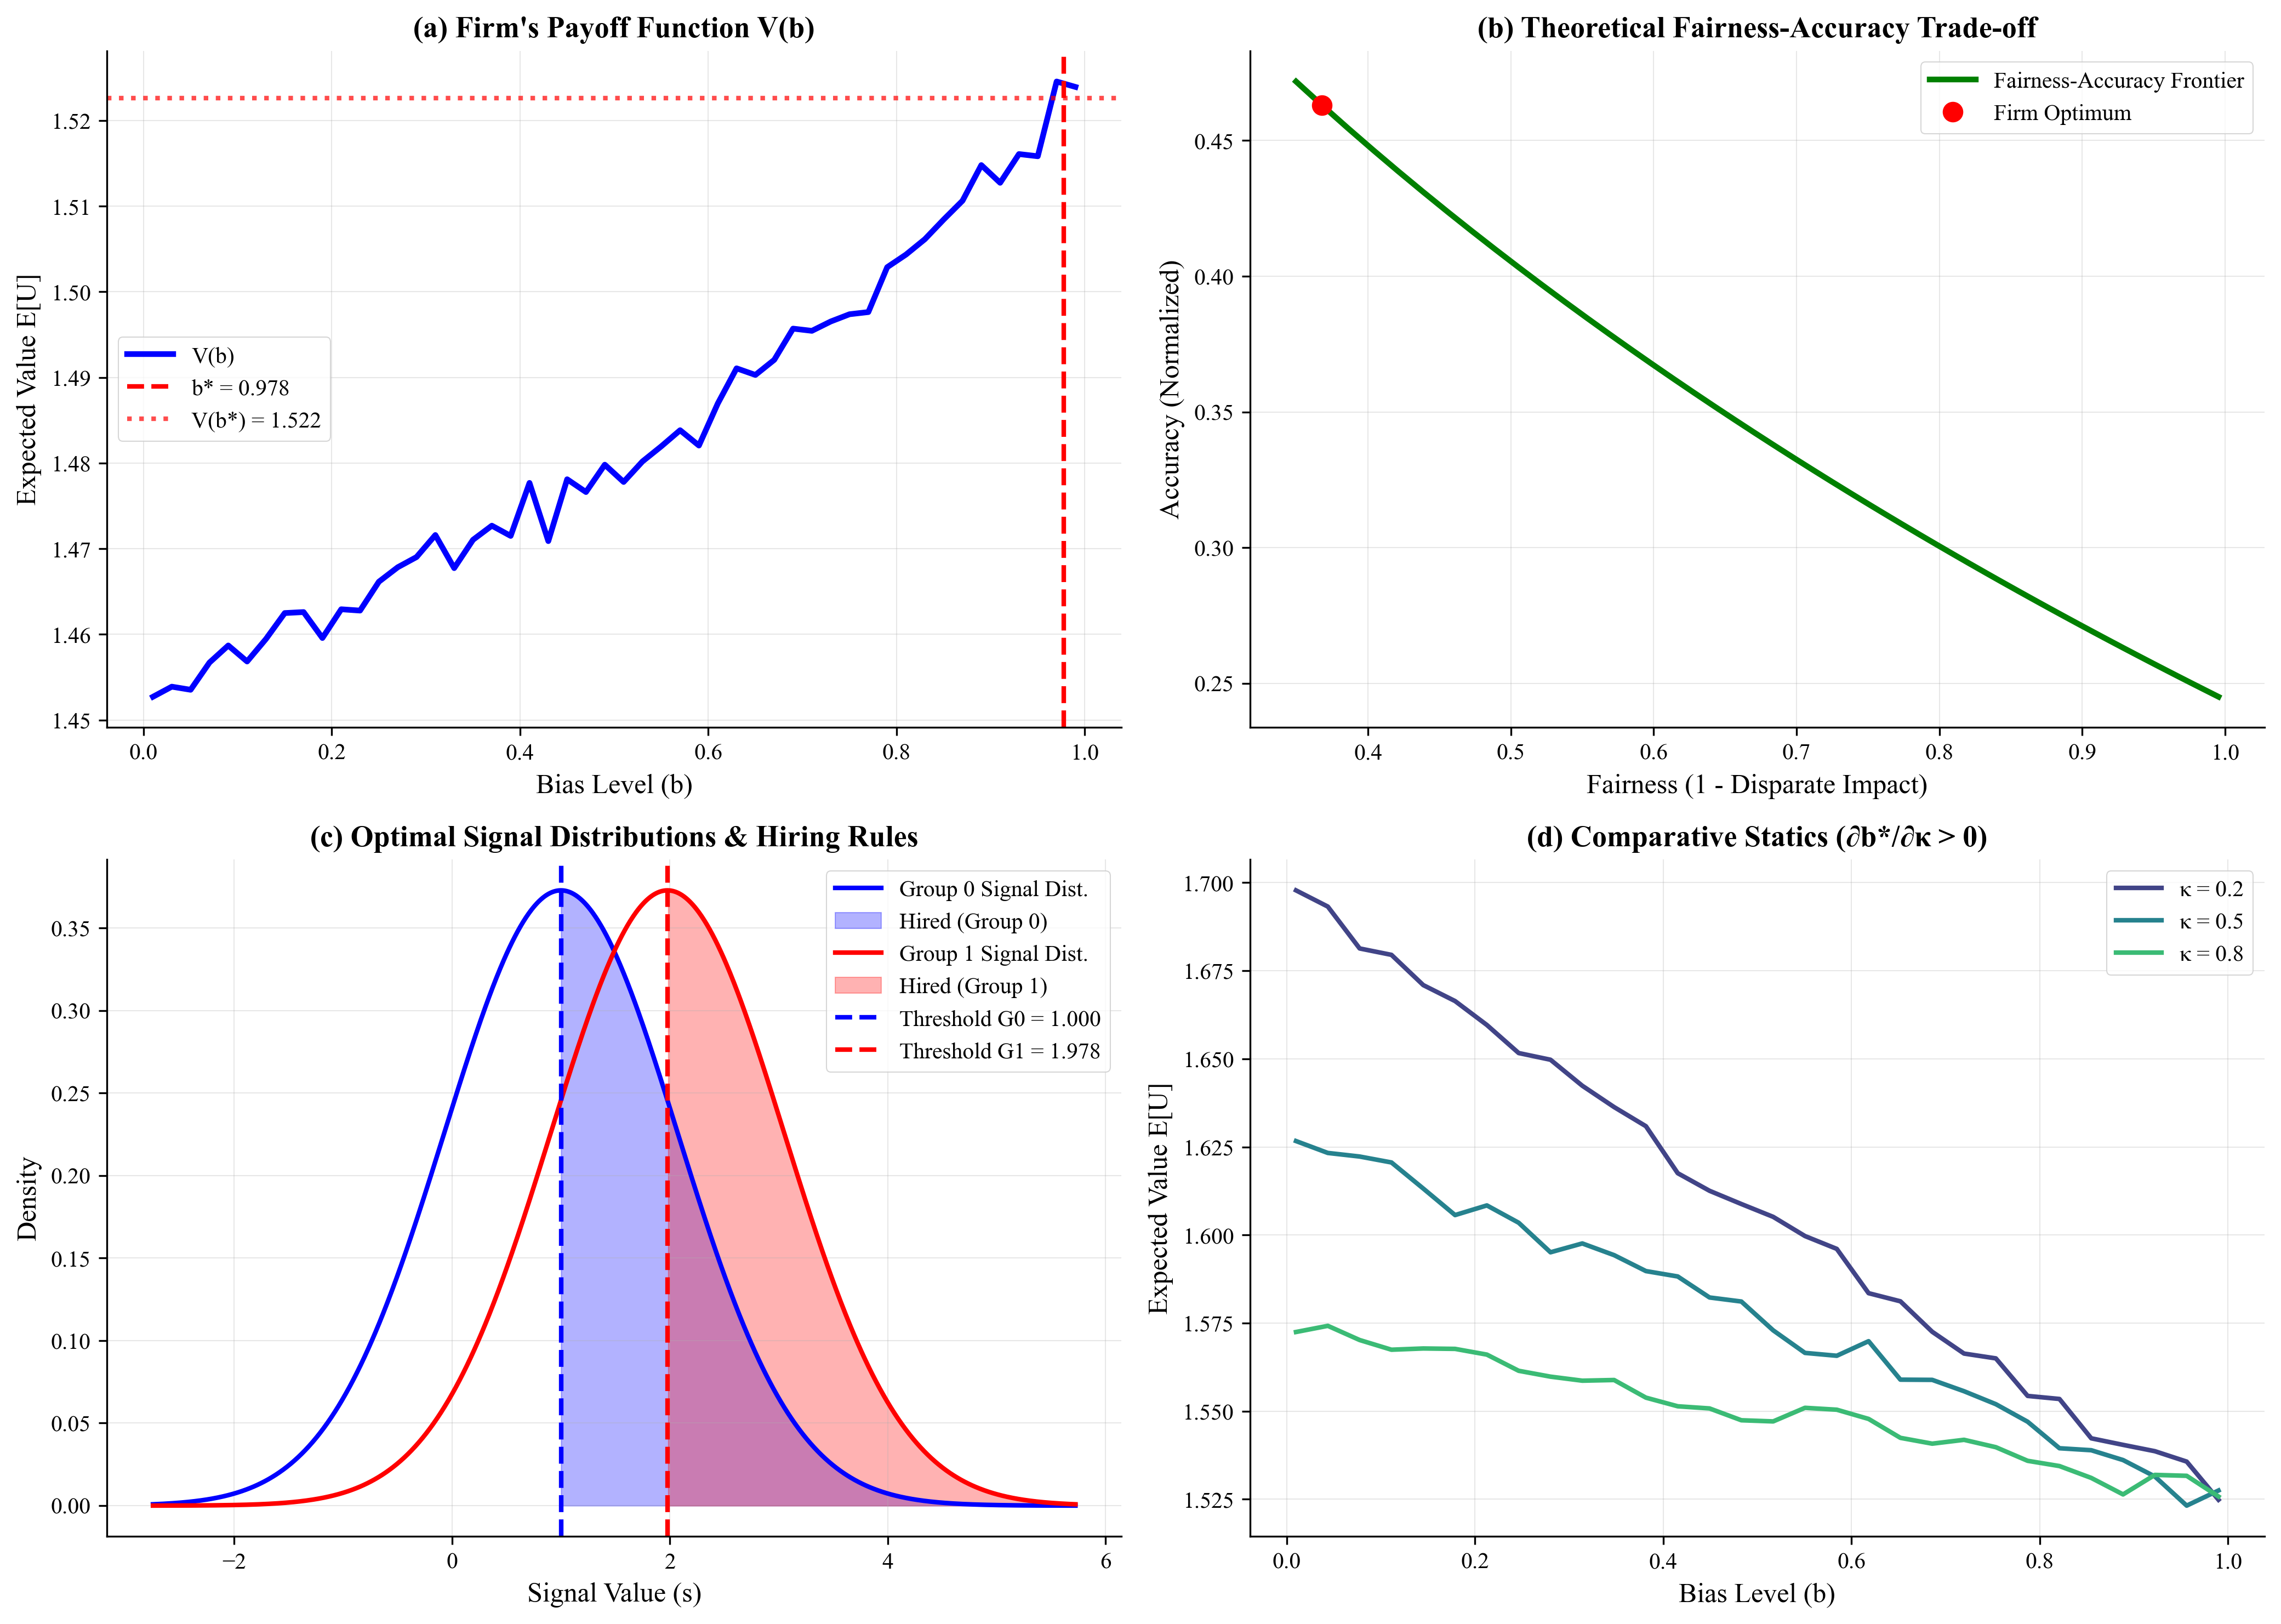
\includegraphics[width=\textwidth]{../figures/figure_1_model_mechanics.png}
    \caption[Model Mechanics and Results]{\textbf{Model Mechanics and Results.} 
    Panel (a): The firm's simulated value function $V(b)$ is maximized at a strictly positive bias $b^*=0.978$. 
    Panel (b): The corresponding fairness-accuracy frontier, with the firm's privately optimal choice marked. 
    Panel (c): The optimal signal distributions for Group 0 (blue) and Group 1 (red). The firm's rational response to bias $b^*$ is to apply a higher effective hiring threshold to Group 1, creating disparate impact.
    Panel (d): A higher technology trade-off parameter $\kappa$ results in a steeper value function, increasing the marginal benefit of bias and thus leading to a higher optimal $b^*$.}
    \label{fig:main_results}
\end{figure}